\documentclass[xcolor={dvipsnames}]{beamer}

\usepackage{beamerthemesplit}
\usepackage{xcolor}
%\startlocaldefs
%\def\argmin{\mathop{\rm arg\,min}\limits}%
%\def\argmax{\mathop{\rm arg\,max}\limits}%
%\endlocaldefs
\usetheme{CambridgeUS}
%\usetheme{Copenhagen}
\usecolortheme{whale}

\definecolor{mycolor}{RGB}{3,86,66}

\setbeamercolor*{structure}{bg=mycolor!20,fg=mycolor}



\setbeamercolor*{palette primary}{use=structure,bg=lightgray,fg=mycolor}
\setbeamercolor*{palette secondary}{use=structure,bg=mycolor,fg=white}
\setbeamercolor*{palette tertiary}{use=structure,bg=black,fg=white}
\setbeamercolor*{palette quaternary}{bg=black,fg=white}
\setbeamercolor*{titlelike}{use=structure,bg=mycolor,fg=white}

\setbeamercolor{frametitle}{bg=structure,fg=white}

%OTHER THEMES: 
% AnnArbor, Antibes, Bergen, Berkeley, Berlin,
% Boadilla, boxes, CambridgeUS, Copenhagen, Darmstadt,
% default, Dresden, Frankfurt, Goettingen, Hannover,
% Ilmenau, JuanLesPins, Luebeck, Madrid, Malmoe,
% Marburg, Montpellier, PaloAlto, Pittsburgh, Rochester,
% Singapore, Szeged, Warsaw

%SEE http://mike.polycat.net/gallery/beamer-themes


%\setbeamercovered{transparent}
\logo{
\includegraphics[height=1.25cm]{1024px-CalPoly_Seal.png}}


%\parskip = .1in
%\usepackage[scale=.75]{geometry}
%\usepackage{amsmath}
\usepackage{graphicx}
\usepackage{amssymb}
\usepackage{epstopdf}
%\usepackage{graphicx}
\usepackage{setspace}
\usepackage{comment}
%\usepackage[dvipdf]{graphicx}

\hypersetup{
    colorlinks=true,
    linkcolor=blue,
    filecolor=magenta,      
    urlcolor=cyan,
}

%
%\setlength{\oddsidemargin}{0.0in}
%\setlength{\topmargin}{-0.5in}
%\setlength{\headheight}{0.20in}
%\setlength{\headsep}{3ex}
%\setlength{\baselineskip}{2ex}
%\setlength{\textheight}{9in}
%\setlength{\textwidth}{6.4in}
%\renewcommand{\baselinestretch}{1.1}

\newcommand{\ft}{\frametitle}
\newcommand{\bi}{\begin{itemize}}
\newcommand{\be}{\begin{enumerate}}
\newcommand{\ei}{\end{itemize}}
\newcommand{\ee}{\end{enumerate}}


\title[]{Teaching Soft Skills in Data Science Curriculum}
\author[Glanz]{Hunter Glanz, Dennis Sun, and Alex Dekhtyar}
\institute[]{California Polytechnic State University \\ San Luis Obispo, California, USA}
\date{July 31, 2019}

\begin{document}
\frame{\titlepage}

\begin{frame}
\frametitle{Outline}
\tableofcontents
\end{frame}

\begin{frame}
\ft{Our Aim}
\bi
	\item Improve students' abilities to collaborate and communicate with peers or team members.
	\pause
	\item Give students formal training on their (technical) writing skills.
	\pause
	\item Give students formal training on their (technical) oral communication skills.
\ei
\end{frame}

\section{Data Science at Cal Poly}

\begin{frame}
\frametitle{Outline}
\tableofcontents[currentsection]
\end{frame}

\begin{frame}
\frametitle{Statistics at Cal Poly}
\bi
	\item Standalone Statistics Department
	\item Quarter system
\ei
\begin{minipage}[t]{.45\linewidth}
	\vspace{-2.5in}
	\centering
	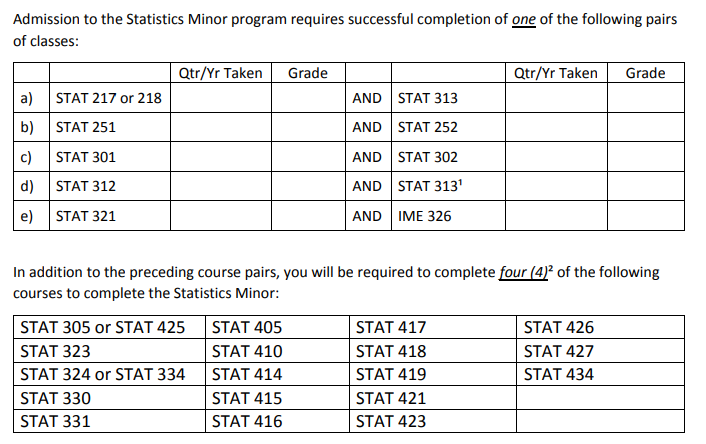
\includegraphics[width = \textwidth]{CP-STAT-minorform.PNG}
\end{minipage}
\begin{minipage}[t]{.45\linewidth}
	\centering
	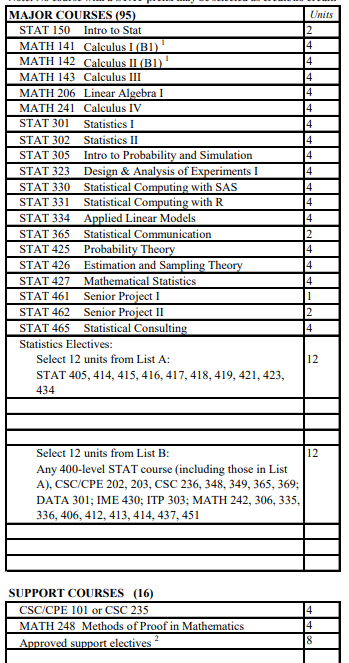
\includegraphics[width = .65\textwidth]{CP-STAT-majorform.PNG}
\end{minipage}
\end{frame}

\begin{frame}
\ft{Cross-Disciplinary Studies Minor in Data Science}
\pause
\bi
	\item \href{https://academicprograms.calpoly.edu/content/academicpolicies/policies-Undergrad/cross-disciplinary-studies-minors}{Cross-Disciplinary Studies Minor} (CDSM):
		\be
			\item Result of partnership between 2+ target major programs.
			\pause
			\item Students gain depth in the partner discipline.
			\pause
			\item Students gain focused study in their own discipline.
			\pause
			\item Students gain focused study in the mutual domain of the minor.
		\ee
	\pause
	\item Our \href{https://statistics.calpoly.edu/data-science-minor}{CDSM in Data Science}:
		\bi
			\item 3-4 years old
			\item Marriage of Statistics and Computer Science
			\item Created by Andrew Schaffner (STAT) and Alex Dekhtyar (CS)
			\item Built primarily for STAT and CS majors, but open to all.
		\ei
\ei
\end{frame}

\begin{frame}
\ft{Cal Poly CDSM in Data Science}
\begin{center}
	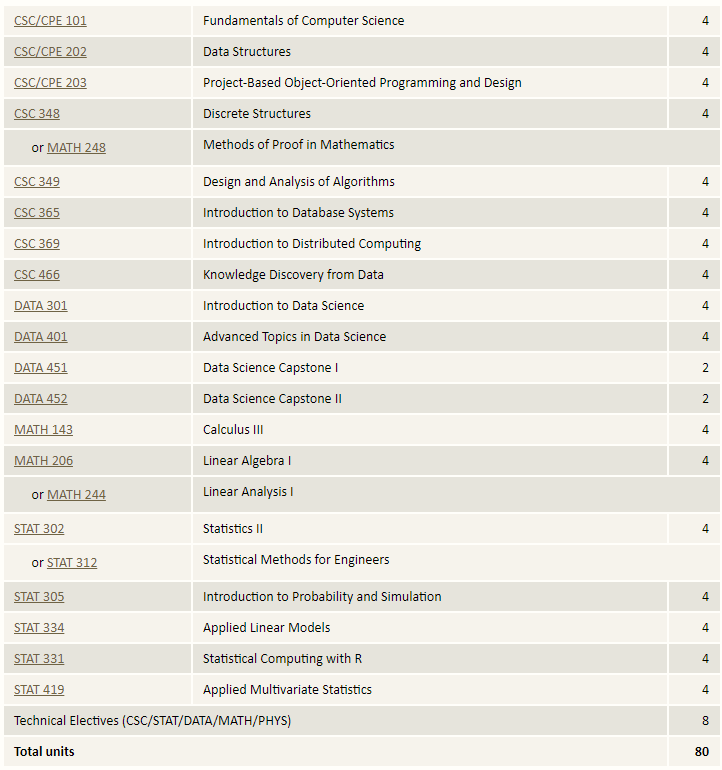
\includegraphics[width = 2.75in]{CP-DS-CDSM-form.png}
\end{center}

\end{frame}

%%%%%%%%%%%%%%%%%%%%%%%%%%%%%%%%%%%%%%%%%%%%%%%%%%%%%%%%%%%%%%%%%%%%%%%%%%%%%%%%%%%%%
\section{Improving Communication Skills}

\begin{frame}
\frametitle{Outline}
\tableofcontents[currentsection]
\end{frame}

\begin{frame}
\ft{Natural Opportunities for Communication Gains}
\pause
\bi
	\item Our data science students work with both R and Python, mostly within the R Markdown/Notebook and Jupyter Notebook interfaces. 
	\pause
	\item Many of the STAT and CS courses involve or accommodate group projects with a presentation and/or write-up component.
	\pause
	\item The DATA courses were newly created with the construction of the CDSM!
\ei
\end{frame}

\begin{frame}
\ft{Senior DATA Sequence}
\pause
\be
	\item DATA 401: Advanced Topics in Data Science
	\pause
		\bi
			\item Mathematical foundations of machine learning
			\item Evolving to include more on ethics and data science culture
		\ei
	\item DATA 451 \& 452: Data Science Capstone I \& II
	\pause
		\bi
			\item Client project-based sequence of two courses
			\item Teams of students engage in data science consulting projects with real clients (both academic and industry) over 20 weeks
		\ei
\ee
\end{frame}

\begin{frame}
\ft{DATA 401: Advanced Topics in Data Science}
\pause
\bi
	\item Natural opportunities continued:
		\bi
			\item Group projects (written and oral deliverables)
			\item Jupyter Notebooks
			\item GitHub
		\ei
	\pause
	
	\item Newer opportunities
		\bi
			\item Peer assessment of assignments
			\item Oral presentation of solutions to homework and in-class activity problems
		\ei
\ei
\end{frame}

\begin{frame}
\ft{DATA 451 \& 452: Data Science Capstone I \& II}
\pause
\bi
	\item Teams of 3-4 students matched with a client for 20 weeks of data science consulting, e.g.:
		\bi
			\item Visualization and analysis of wearable monitor data (Kinesiology and Public Health)
			\pause
			\item Identification of malicious network activity (Industry)
			\item Both local and remote clients
		\ei
	
	\pause
	\item Minimum oral deliverables:
		\bi
			\item 30 minute meetings between team and client every other week (10 total)
			\item Two project presentations: mid-project and project end
		\ei
		
	\pause
	\item Minimum written deliverables:
		\bi
			\item Commented and documented Notebook/code files
			\item Two reports: mid-project and project end
		\ei
\ei
\end{frame}

\begin{frame}
\ft{Boosting Oral Communication}
\bi
	\item Borrowing from STAT 465 (our consulting course) and beyond!
\ei
\begin{center}
	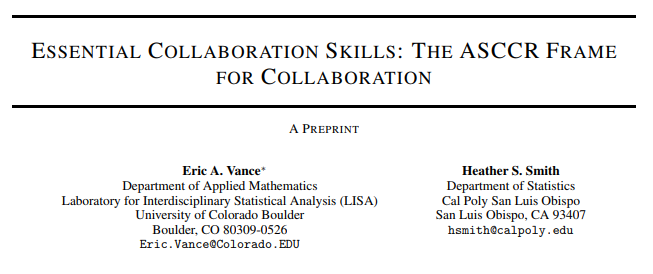
\includegraphics[width = .55\textwidth]{HSmith_ASCCR_paper.png}
\end{center}
\begin{center}
	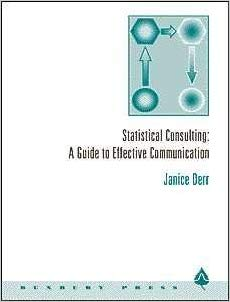
\includegraphics[width = .2\textwidth]{STAT465book.jpg}
	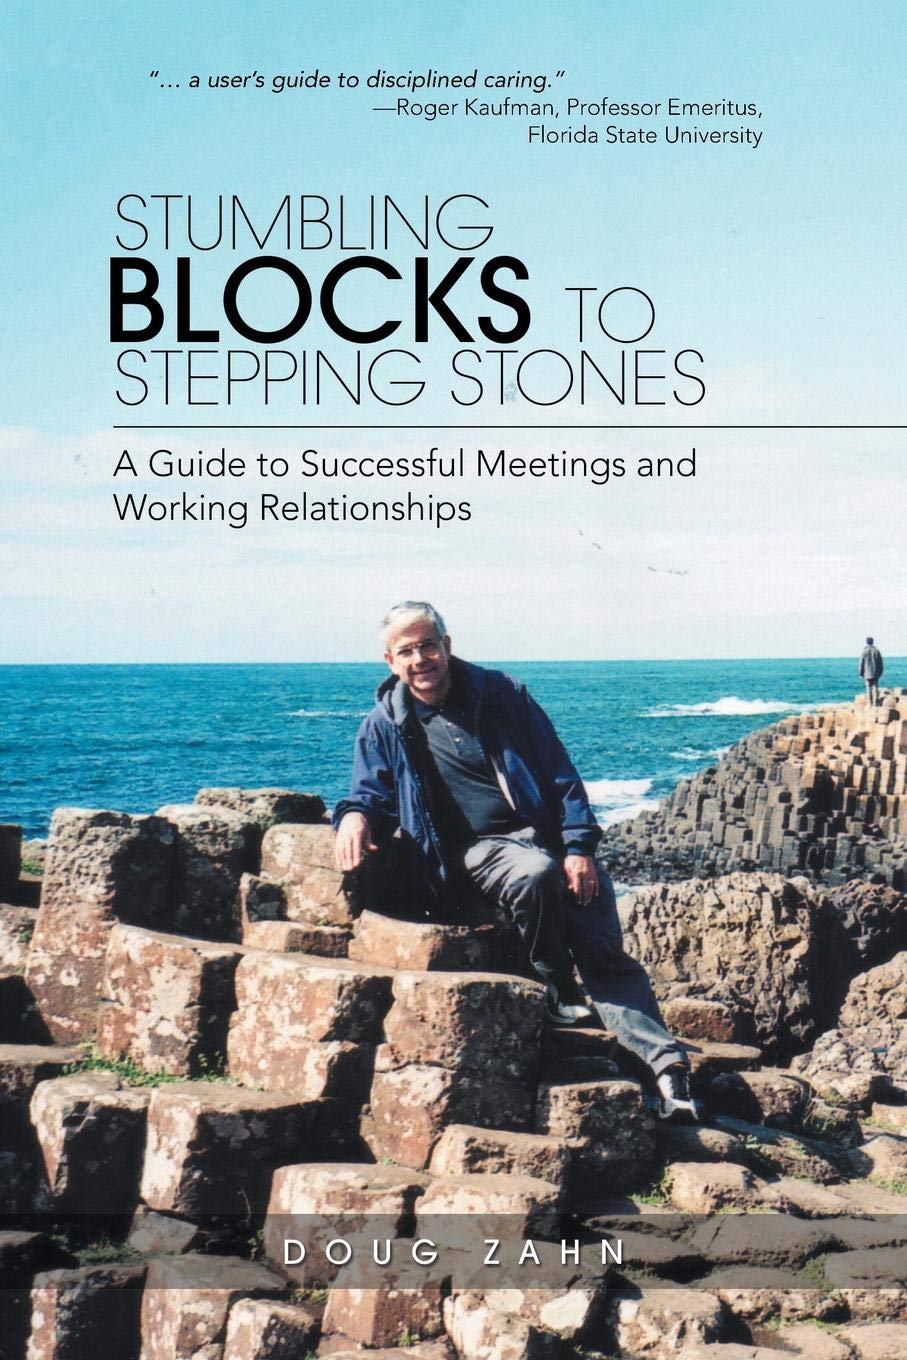
\includegraphics[width = .2\textwidth]{DougZahnbook.jpg}
\end{center}
\end{frame}

\begin{frame}
\ft{Boosting Written Communication}
\bi
	\item Applying lessons in style and grace to their own reports from DATA 401 and eventually DATA 451!
	\pause
	\item Oral presentations of their revisions accompanied by discussions of the lessons themselves.
\ei
\begin{center}
	
\includegraphics[width = .25\textwidth]{styleandgrace_book.jpg}
\end{center}
\end{frame}

%%%%%%%%%%%%%%%%%%%%%%%%%%%%%%%%%%%%%%%%%%%%%%%%%%%%%%%%%%%%%%%%%%%%%%%%%%%%%%%%%%%%%%
\section{Conclusion}

\begin{frame}
\ft{Conclusion}
\bi
	\item Improve students' abilities to collaborate and communicate with peers or team members.
	\pause
	\item Give students formal training on their (technical) writing skills.
	\pause
	\item Give students formal training on their (technical) oral communication skills.
\ei
\end{frame}

\begin{frame}
\frametitle{Thank You! Questions?}
\begin{center}
	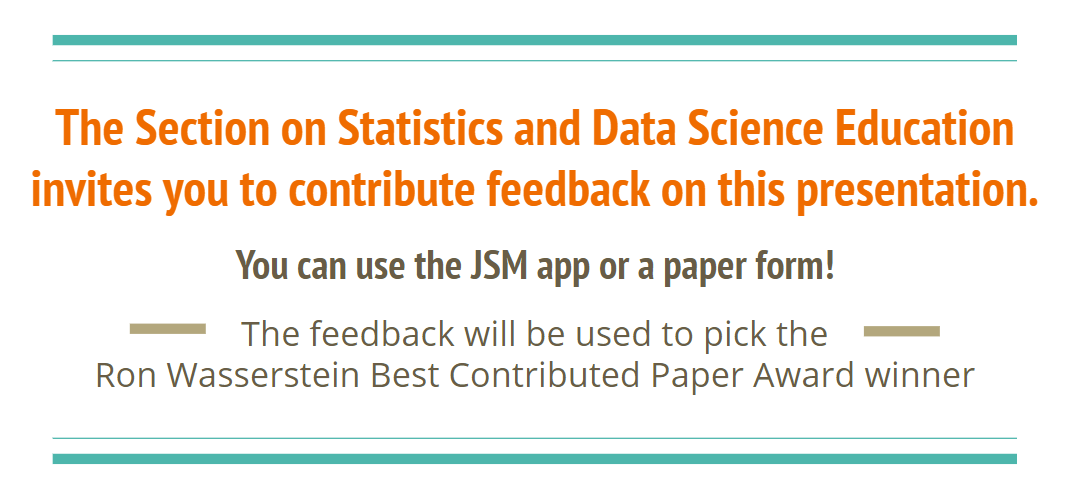
\includegraphics[width = 4in]{lastslide_survey.png}
\end{center}
\end{frame}


\end{document}